\chapter{O \textit{Clean Pool Robot}} \label{ch:cpr}
\section{Visão Geral}
O \cpr é um equipamento que visa auxiliar a limpeza de grandes piscinas, como os modelos semiolímpicos. O robô faz a aspiração e filtragem das impurezas presentes no fundo da piscina, removendo as algas e folhas e auxiliando na circulação da água. O mecanismo do mesmo será composto por dois métodos para que o fundo da piscina possa ser aspirado: o primeiro baseia-se na escovação do chão e o segundo a sucção das impurezas desprendidas do piso da piscina.

O primeiro método tem foco nas escovas que estão situadas na parte inferior do robô. As escovas realizam movimentos giratórios fazendo com que suas cerdas entrem em contato com o chão retirando  impurezas, como por exemplo: algas e grãos de terra.

Após a escovação, é realizado outro método, a sucção das impurezas desprendidas do piso da piscina  além de outras impurezas que estiverem próximas à área de atuação do robô, por exemplo: pequenos ramos e folhas. Por meio de uma bomba, a água é sugada por uma abertura situada na parte inferior e passa por um filtro. As impurezas menores ficam retidas no filtro. Por meio de um sistema de expulsão de água, esta sairá a uma velocidade muito superior à velocidade de entrada no início do processo, ajudando na movimentação do robô.

Com o término da limpeza na piscina, haverá a necessidade dos filtros serem limpos para retirada das impurezas colhidas na aspiração da água. Assim, após cada utilização o usuário deverá limpar os filtros internos do \cpr.

O produto desenvolvido será responsável apenas pela retirada da sujeira decantada no fundo da piscina, ou seja, o \cpr não limpará as paredes ou superfície da piscina. Além disso, as piscinas ideais para a operação do robô são as retangulares, sem inclinações e azulejadas. É ideal também que o robô seja lançado na piscina no meio da largura maior, evitando que o fio fique totalmente esticado quando o robô estiver na quina oposta do lançamento.

\section{O \textit{Design}}
A Figura \ref{fig:croqui-design-cpr} mostra o \cpr projetado no \software Catia. O modelo apresenta dois rolos de limpeza, localizados na parte frontal e traseira do robô, um duto, na parte superior para a saída da água filtrada, que também funciona como propulsão e direcionador dos movimentos do robô. A sucção da água feita por meio das duas aberturas na parte inferior do robô. Abaixo a figura com croqui do design do \textit{Clean Pool Robot}.
\par
  \begin{figure}[h]
    \centering
    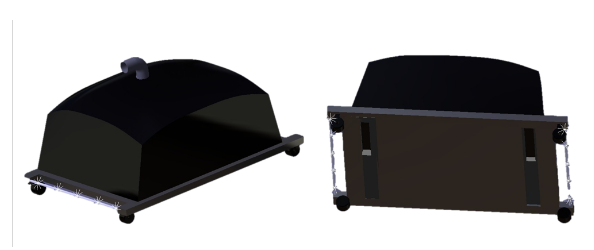
\includegraphics[width=0.8\textwidth]{figures/croqui-design-cpr.png}
    \caption{Croqui com o design do \textit{Clean Pool Robot}, vista frontal e inferior.}
    \label{fig:croqui-design-cpr}
  \end{figure}
  \FloatBarrier
\par
Por motivo de resistência ao movimento o formato do robô foi modificado para melhor aproveitamento das forças hidrodinâmica envolvidas, as alterações no desenho inicial foram feitas com a intenção de diminuir a força de arrasto, a estrutura conta agora com cantos e arestas arredondadas conforme a Figura \ref{fig:croqui-design-cpr}.

O \textit{design} apresentado é a segunda versão, em que foi melhorado o posicionamento das escovas. Nessa versão elas ficam na extremidade do robô, onde auxiliam em eventuais impactos (por mais que seja pequeno) do robô com a parede.

\section{Sistemas}
O Robô possui três principais sistemas para o seu funcionamento: o Sistema de Automação, composto pelos sensores e programações lógicas de acionamento, Sistema de Locomoção, formado pelo conjunto das rodas, bomba e motores, e o Sistema de Limpeza, com os filtros e rolos de limpeza. A Figura \ref{fig:main-system-project} mostra os três sistemas e a relação entre eles.
\par
  \begin{figure}[h]
    \centering
    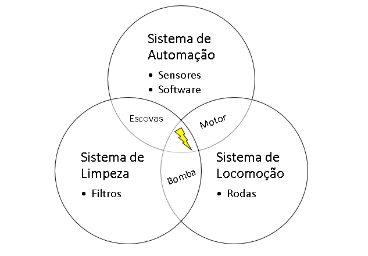
\includegraphics[width=0.8\textwidth]{figures/main-system-project.png}
    \caption{Três principais sistemas do Robô: Automação, Limpeza e Locomoção.}
    \label{fig:main-system-project}
  \end{figure}
  \FloatBarrier
\par

\section{Indicadores}
Os indicadores de desempenho são métricas que quantificam a performance de acordo com os objetivos propostos. Para auxiliar a validação da verificação da limpeza do robô, determinou-se um indicador que é o \textsf{CDL} - Ciclo de Limpeza.

O \textsf{CDL} faz uma avaliação da limpeza em gruas de leve até uma limpeza minuciosa. O parâmetro para a avaliação do cliclo se faz em comparação com tempo, caso a duração total da limpeza seja menor que 5h, então o robô terá executado um \textsf{CDL} leve, ou seja, limpeza rápida e mais leve. Esse \textsf{CDL} é indicado para piscinas que estejam, por inspeção visual, com pouca sujeita depositada ao fundo.

Caso o tempo total da limpeza seja maior que 5h, o \textsf{CDL} utilizado foi equivalente a uma limpeza minuciosa. Neste caso a piscina deve estar com maior quantidade de impurezas depositadas ao fundo. A Figura \ref{fig:indicator} mostra a represenatção do indicador.
\par
  \begin{figure}[h]
    \centering
    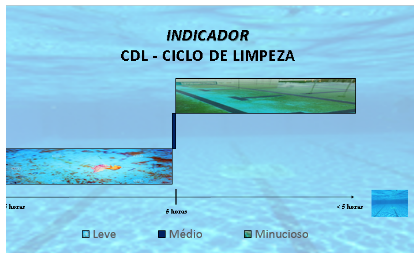
\includegraphics[width=0.8\textwidth]{figures/indicator.png}
    \caption{Indicador CDL.}
    \label{fig:indicator}
  \end{figure}
  \FloatBarrier
\par

\section{Custos}
No desenvolvimento do \cpr foram gastos até o momento os valores apresentados na tabela abaixo. Considerando um lucro de 10\% sob cada peça, o custo estimado para a venda do Robô é de R\$ 6.500, estando comercialmente competitivo.
\begin{table}[h]
\centering
\caption{Valores de Custos do \textit{Clean Pool Robot}}
\label{my-label}
\begin{tabular}{@{}cc@{}}
Carga horária máxima                      & 90 h         \\
Valor da Hora (Valor da Capes – Graduado) & R\$ 24, 44   \\
Pessoas no desenvolvimento do produto     & 12           \\
Hora por mês                              & 20           \\
Preço total da mão de obra                & R\$ 5.866,67 \\
Material                                  & R\$ 1.349,50 \\
Lucro                                     & 10\%         \\ \midrule
Valor total para Venda (sem impostos)     & R\$ 6.494,55
\end{tabular}
\end{table}

Uma pesquisa realizada apresentou o custo dos principais concorrentes do Clean Pool Robot que está entre R\$ 2.000,00 e R\$ 16.000,00, assim o valor de mercado está dentro da classe dos produtos mais baratos.
